% !TEX root = ../report.tex
\section{Die Physik}
\begin{Spacing}{\mylinespace}
    Die Physik soll eine möglichst echtzeitfähige und
    realitätsgetreue Simulation von Luftströmung über eine dynamische Landschaft berechnen.
    Zu diesem Zweck sollten die Partikel des Partikelsystem die einzelnen
    Luftteilchen darstellen und mithilfe einer einfachen Physik
    die Interaktion zwischen diesen und ihrer Umgebung simuliert werden.
    \subsection{Komponenten}
        Jedes Luftpartikel besteht aus zwei dreidimensionalen Vektoren.
        Der Vektor $\vec{p}_{i}$ stellt dabei die Position des Partikels im
        Raum dar und der Vektor $\vec{v}_{i}$ beschreibt die aktuelle Bewegung des Partikels.
        Außerdem besitzen alle Partikel den gleichen Radius $r$ und einem
        Reibungskoeffizienten $\mu$, welcher bestimmt wie viel Energie ein Partikel
        bei einer Kollision verliert.
        Zusätzlich zu den Partikeln stehen Informationen über die Umgebung
        wie z.B. Höhendaten der Landschaft und verschiedene externe
        Kräfte ($F$), wie z.B. Gravitation, zur Verfügung.

        %\[ P_{i} = ( \vec{p}_{i}, \vec{v}_{i} ) , P_{i} \in P \]
        %\[ \vec{p}_{i} \in \mathbb{R}^{3} \]
        %\[ \vec{v}_{i} \in \mathbb{R}^{3} \]

        %\[ h_{xy} \in \mathbb{R} \]
        %\[ \vec{f}_i \in \mathbb{R}^{3} \]

    \subsection{Bewegung der Partikel}
        Um die Bewegung der Partikel zu simulieren wird in jeder Iteration,
        für jedes einzelne Partikel, der Bewegungsvektor $\vec{v}_{i}(t)$
        auf den Positionsvektor $ \vec{p}_{i}(t)$ aufaddiert.

        \[ \vec{p}_{i}(t+1) = \vec{p}_{i}(t) + \vec{v}_{i}(t) \]

        Auf diese Weise wird der Impuls solange erhalten bis der Bewegungsvektor
        durch Einwirkung äußerer Kräfte verändert wird.

        \begin{figure}[h!]
			\centering
			\vspace*{30px}
			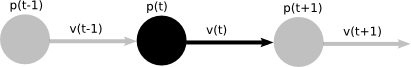
\includegraphics[width=0.7\textwidth]{graphics/Phys_bew0.png}
			\caption{Konstante Bewegung}
			\label{fig:BewegungPartikel}
		\end{figure}

		In diesem Fall wird angenommen das der zeitliche Abstand zwischen den
		einzelnen Iterationen konstant ist. Wenn die Dauer zwischen den Iterationen
		schwankt ist es ratsam dies zu kompensieren indem man den Bewegungsvektor
		$\vec{v}_{i}$ mit dem zeitlichen Abstand ($\Delta t$) zwischen den
		Iterationen multipliziert.
		 \[ \vec{p}_{i}(t+\Delta t) = \vec{p}_{i}(t) + \vec{v}_{i}(t) * \Delta t\]

    \subsection{Verrechnung externer Kräfte}
        In jeder Iteration wird die Wirkung externer Kräfte ($F$) auf das
        Partikel berechnet. Dabei wird jede der externen Kräfte ($\vec{f}_i$) auf den
        Bewegungsvektor $\vec{v}_{i}(t)$ aufaddiert.

        \[ \vec{v}_{i}(t+1) = \vec{v}_{i}(t) + \sum_{\vec{f}_{i} \in F}{\vec{f}_{i}} \]

		\begin{figure}[h!]
			\centering
			%\subfigure(1){ 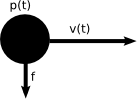
\includegraphics[width=0.2\textwidth]{graphics/Phys_bew1.png} \label{fig:ModForce1} }
			%\subfigure(2){ 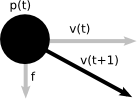
\includegraphics[width=0.2\textwidth]{graphics/Phys_bew2.png} \label{fig:ModForce2} }
			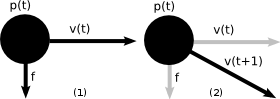
\includegraphics[width=0.4\textwidth]{graphics/Phys_bew12.png}
			\caption{Bewegungsvektor vor(1) und nach(2) Modifikation durch eine externe Kraft }
			\label{fig:ModForce}
		\end{figure}

        Eine externe Kraft ist beispielsweise die Gravitation, welche die Partikel
        in die untere Richtung beschleunigt. Diese Wirkung kann dadurch erzielt
        werden indem beispielsweise der Vektor $( 0,-9.81,0 )$ zu der Menge der externen
        Kräfte hinzufügt wird.
		Diese schrittweise Aufaddierung führt, über mehrere Iteration hinweg gesehen,
		zur Beschleunigung des Partikels, wie es in der Abbildung \ref{fig:bewmod} dargestellt wird.
		\begin{figure}[h!]
			\centering
			\vspace*{30px}
			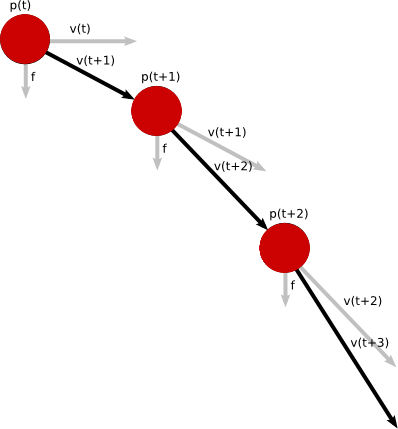
\includegraphics[width=0.7\textwidth]{graphics/Phys_bew3.png}
			\caption{Die auf das Partikel wirkende Kraft(f) bleibt konstant und
			die Bewegung wird bei jedem Rechenschritt weiter in die Richtung der
			Kraft beschleunigt}
			\label{fig:bewmod}
		\end{figure}

    \subsection{Kollisionserkennung von Partikeln mit der Umgebung}
    	Nachdem ein Partikel bewegt wurde, wird überprüft ob eine Kollision mit
    	der Heightmap vorliegt. Eine Kollision liegt vor wenn die vertikale Komponente
    	des Positionsvektors des Partikels einen niedrigeren Wert enthält als der
    	Höhenwert der Heightmap unterhalb der horizontalen Position des Partikels. Wenn dieser Fall
    	vorliegt befindet sich das Partikel unterhalb der Heightmap und ist
    	folglich während der letzten Positionsänderung in das Terrain eingedrungen
    	und es liegt nun eine Kollision vor.

    	Zusätzlich kann der Durchmesser des Partikels berücksichtigt werden
    	indem man den Radius zu dem Höhenwert der Heightmap aufaddiert und
    	dadurch eine Kollision erkannt wird bevor der Positionsvektor unterhalb
    	der tatsächlichen Heightmap liegt.

    \subsection{Kollisionsauflösung von Partikeln mit der Umgebung}
    	Wurde erkannt dass das Partikel mit der Heightmap kollidiert ist, wird eine
    	Kollisionsauflösung durchgeführt. Dabei wird zuerst die Flächennormale
    	der Heightmap ($\vec{n}$) an dem Ort der Kollision berechnet.

    	%\[ \vec{n} = float3((s1 - s3) * coef, 2.0f, (s2 - s4) * coef); \]

    	Mithilfe der Flächennormale $\vec{n}$ wird nun die Reflektion des Bewegungsvektor
    	berechnet und die Bewegungsrichtung auf diese Weise verändert.

    	\[ \vec{v}_{i}(t+1) = \vec{v}_{i}(t+1) -2 \cdot \langle \vec{v}_{i}(t+1) , \vec{n} \rangle \cdot \vec{n} \]

		\begin{figure}[h!]
		%\centering{
			%\subfigure(1){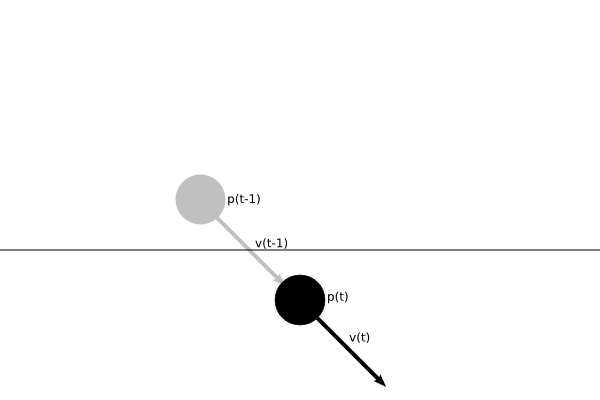
\includegraphics[width=0.4\textwidth]{graphics/Phys_kh1.png}}
			%\subfigure(2){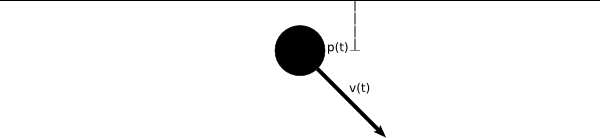
\includegraphics[width=0.4\textwidth]{graphics/Phys_kh2.png}}
			%\subfigure(2){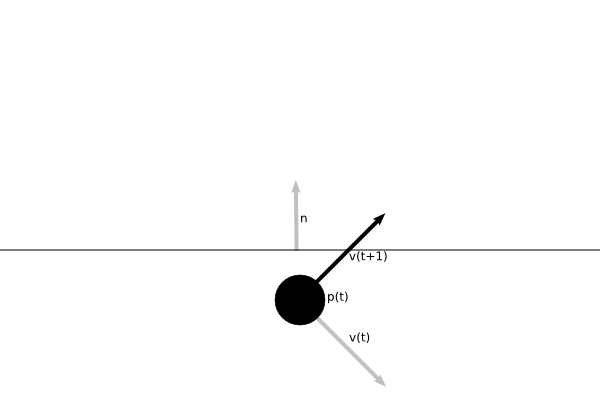
\includegraphics[width=0.4\textwidth]{graphics/Phys_kh3.png}}
			%\subfigure(2){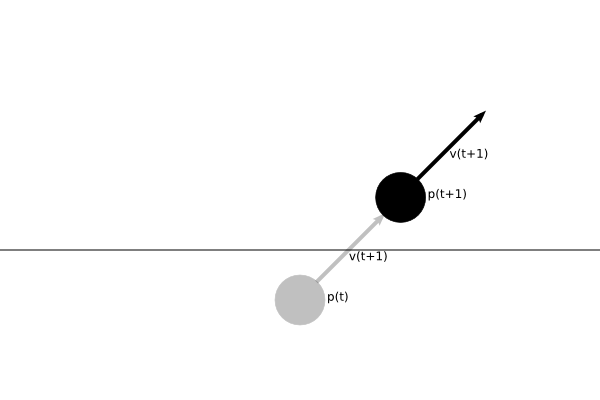
\includegraphics[width=0.4\textwidth]{graphics/Phys_kh4.png}}}
			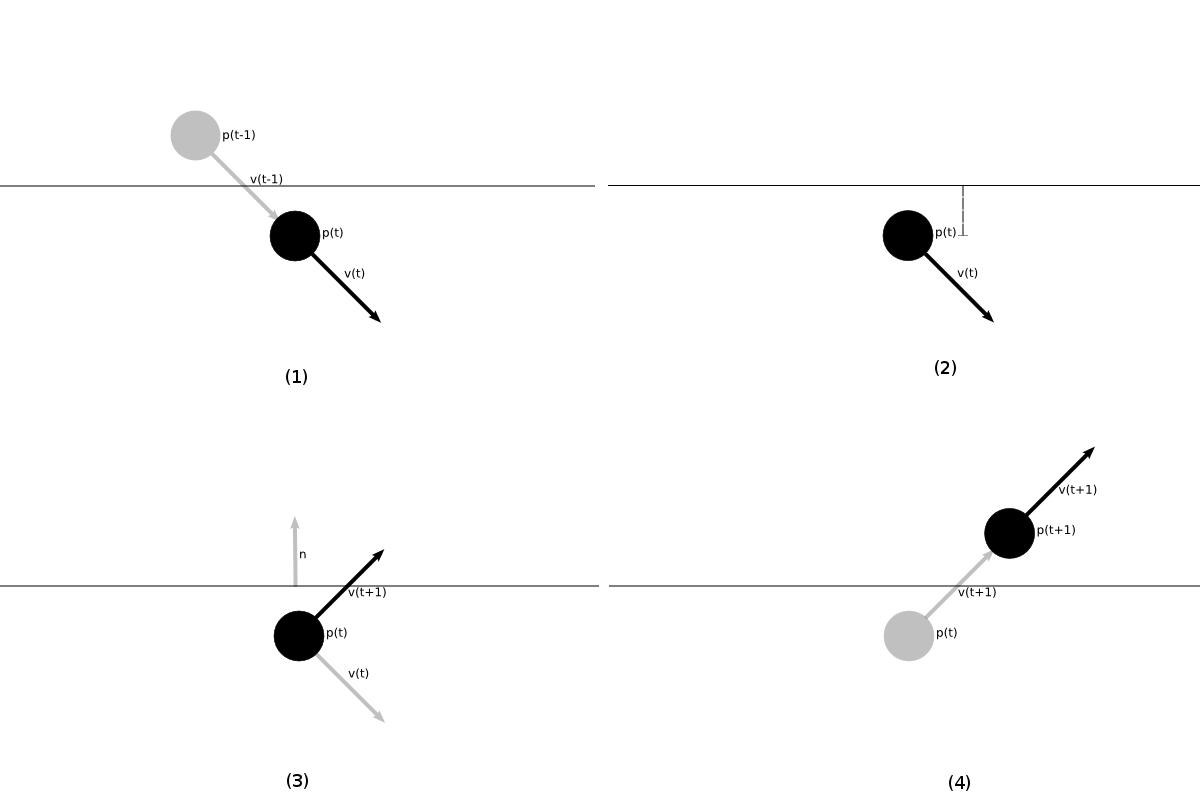
\includegraphics[width=0.99\textwidth]{graphics/Phys_kh1234.png}
			\caption{(1) Partikel dringt in die Heightmap ein. (2) Erkennung der Kollision. (3) Reflektion des Bewegungsvektors(v) entlang der Flächennormale(n). (4) }
			\label{fig:reflexHeihtmap}
		\end{figure}

		Allein mithilfe der Reflektion können bereits die meisten Kollisionen
		aufgelöst werden. Wenn beispielsweise ein Partikel senkrecht zur Oberfläche
		in die Heightmap eindringt wird der Bewegungsvektor auf diese Weise umgekert
		und das Partikel wird sich in der nächsten Iteration wieder aus der Heightmap
		herausbewegen.
		%\[ \vec{v}_{i}(t) = \left(\begin{array}{rr} 0 \\ 0 \\0 \end{array}\right) , \vec{f}_{i} = \left(\begin{array}{rr} 0 \\ -1 \\0 \end{array}\right) , \vec{n} = \left(\begin{array}{rr} 0 \\ 1 \\0 \end{array}\right) \]
		%\[ \vec{v}_{i}(t+1) = \left(\begin{array}{rr} 0 \\ -1 \\0 \end{array}\right) -2 \cdot \langle \left(\begin{array}{rr} 0 \\ -1 \\0 \end{array}\right) , \left(\begin{array}{rr} 0 \\ 1 \\0 \end{array}\right) \rangle \cdot \left(\begin{array}{rr} 0 \\ 1 \\0 \end{array}\right) = \left(\begin{array}{rr} 0 \\ 1 \\0 \end{array}\right) \]
		\\Die Kombination aus Reflektion und Gravitation führt außerdem dazu, dass
		Partikel die auf der Heightmap liegenbleiben sind, sich entlang des Gefälles
		der Heightmap bewegen, oder im Falle einer horizontalen Ebene auf der aktuellen Position liegenbleiben.
		Dies wird dadurch verursacht, dass ein liegengebliebenes
		Partikel einen Nullvektor als Bewegungsvektor besitzt, wodurch nach Verrechnung der
		Gravitation der Bewegungsvektor dem Vektor der Gravitation entspricht und
		verursacht dass das Partikel in die Heightmap bewegt wird, wodurch eine Kollision hervorgerufen wird.
		Wenn die Flächennormale in die entgegengesetzte Richtung der Gravitation
		zeigt, wie es im Fall einer horizontalen Ebene vorliegt, wird der
		Bewegungsvektor durch die Reflektion vollständig umgekehrt.
		In der nächsten Iteration wird das Partikel wieder an seine
		Ursprungsposition bewegt und die Addition der Gravitation zum Bewegungsvektor führt zur
		Neutralisierung der Bewegung, wodurch der Bewegungsvektor wieder
		zu einem Nullvektor wird und somit die Ausgangssituation wiederhergestellt ist.

		Wenn allerdings die Kollision an einem Gefälle stattfindet, neutralisieren
		sich Bewegung und Gravitation nur teilweise. Da die Gravitation keinen
		Einfluss auf den horizontalen Anteil der Bewegung hat, bleibt dieser
		erhalten und das Partikel bewegt sich in der nächsten Iteration in die
		horizontale Richtung der Flächennormale.
		Auf diese Weise bewegen sich Partikel auf der Oberfläche der Heightmap
		und folgen dabei der horizontalen Richtung der aktuellen Flächennormale.
		Bei einem Gefälle führt dieser Vorgang dazu, dass die Partikel sich,
		wie in Abbildung \ref{fig:rolling} dargestellt ist,
		entlang der schiefen Oberfläche nach unten bewegen, bis sie schließlich
		in einem Tal liegenbleiben. Oder im Fall einer horizontalen Ebene auf der Oberfläche liegenbleiben.
		\begin{figure}[h!]
			\centering
			\vspace*{30px}
			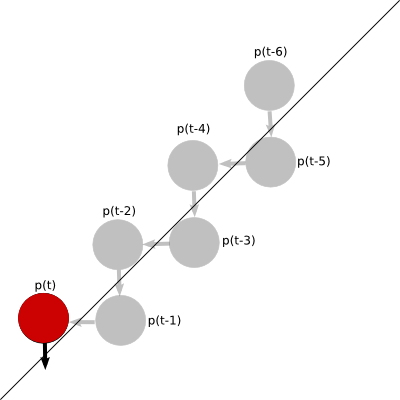
\includegraphics[width=0.7\textwidth]{graphics/Phys_rolling.png}
			\caption{Bewegung eines Partikels entlang eines Gefälles.}
			\label{fig:rolling}
		\end{figure}


		Nach der Reflektion kann die Reibung einbezogen werden, indem der Bewegungsvektor
		$\vec{v}_{i}$ von dem Reibungskoeffizienten $\mu$ gekürzt wird. Wobei $\mu$
		einen festen Wert zwischen 0 und 1 besitzen muss und für alle Partikel gleichermaßen gilt.
		\[ \vec{v}_{i}(t+1) = \vec{v}_{i}(t+1) \cdot ( 1 - \mu ) \]
		Bei dem Wert 1 würde das Partikel alle Bewegungsenergie verlieren und auf der
		Aufprallstelle liegenbleiben. Je kleiner dieser Wert jedoch ist desto weniger
		Energie geht bei einer Kollision verloren und ein Wert von 0 führt dazu, dass
		die Reibung keinen Einfluss mehr auf den Bewegungsvektor hat.

		Die Reibung sorgt dafür, dass die Partikel bei jeder Kollision immer langsamer
		werden, bis sie schließlich vollständig zum erliegen kommen und
		nicht dauerhaft ungebremst und durch die gesamte Welt springen.
		Der Verlust von Bewegungsenergie bedeutet allerdings auch, dass bei einem auf der
		Landschaft liegengebleibenes Partikel die Reflektion nicht mehr vollständig die
		Gravitation ausgleichen kann. Der Bewegungsvektor würde in der
		nächsten Iteration entgegen der Gravitation zeigen, dieser ist allerdings durch die Reibung
		schwächer als die Gravitation und kann diese nun nicht mehr vollständig neutralisieren. Die Reflektion
		reicht nun durch die Kombination mit der Reibung, nicht mehr alleine aus
		um zu verhindern, dass liegengebliebe Partikel immer weiter in die Oberfläche eindringen.

		Um dies zu verhindern wir ein weiterer Mechanismus bei der Kollisionsauflösung benötigt.



    \subsection{Kollisionserkennung zwischen Partikeln}
    	Um eine Kollision zwischen zwei Partikeln festzustellen errechnet man
    	den Abstand zwischen beiden indem man beide Positionsvektoren voneinander
    	subtrahiert und den Betrag des daraus resultierenden Vektors ermittelt.
    	Wenn alle Partikel kugelförmig sind und den gleichen Durchmesser besitzen
    	lässt sich eine Kollision sehr einfach ermitteln indem man den Abstand
    	zwischen den Partikeln mit dem doppelten Radius der Partikel vergleicht.
    	\[ \vert \vec{p}_{i} - \vec{p}_{j} \vert \leq 2r \rightarrow \textrm{Kollision liegt vor} \]
    	\[ \vert \vec{p}_{i} - \vec{p}_{j} \vert > 2r \rightarrow \textrm{Keine Kollision} \]
    	Solange der Abstand zwischen beiden Partikeln größer ist als der
    	doppelte Radius liegt keine Kollision vor.
    \subsection{Kollisionsauflösung zwischen Partikeln}
    	Wenn eine Kollision zwischen Partikeln festgestellt wurde, kann diese in
    	ähnlicher Weise aufgelöst werden wie eine Kollision mit der Landschaft.
    	Dabei
    \subsection{Übertragung der Kräfte zwischen Partikeln}
\end{Spacing}
\newpage
\clearpage
%% End Of Doc
